\documentclass{beamer}

\usepackage{mathtools,amsthm,cancel}
\DeclarePairedDelimiter\ceil{\lceil}{\rceil}
\DeclarePairedDelimiter\floor{\lfloor}{\rfloor}

\newcommand*{\mycite}[1]{~\cite{#1}}

\usepackage{hyperref}

\usepackage{biblatex}
\addbibresource{cites.bib}

% 
% A FLAME algorithm is bracketed by
%
%  \begin{FlameAlg}
%    <statements>
%  \end{FlameAlg}

\newenvironment{FlameAlg}{
\begin{tabbing}
in \= in \= in  \= in  \= in  \= \kill
}
{
\end{tabbing}
}

\newboolean{IsWide}
\setboolean{IsWide}{true}

\newenvironment{FlameAlgNarrow}{
\setboolean{IsWide}{false}
\begin{tabbing}
in \= in \= in  \= in  \= in  \= \kill
}
{
\end{tabbing}
\setboolean{IsWide}{true}
}

%
% A loop in a FLAME algorithm is bracketed by
%
% \FlaDoUntil{ <condition> }
%   Body of the loop
% \FlaEndDo
%
% The body is indented

\newcommand{\FlaDoUntil}[1]{
{ \bf do until #1 } \+ 
}

% Note: because of the \kill, it is important
% to have a \\ before the \FlaEndDo
% since otherwise the last line before the
% \FlaEndDo will not show

\newcommand{\FlaEndDo}{
\- \kill
{ \bf enddo }
}

% In math mode, 
% \FlaTwoByTwo{A}{B}
%             {C}{D}
% creates the picture
%   / A || B \
%   | ==  == |
%   \ C || D /

\newcommand{\FlaTwoByTwo}[4]{
\left( 
\begin{array}{c || c}
#1 & #2 \\ \hline \hline
#3 & #4 
\end{array} 
\right)
}

\newcommand{\FlaTwoByTwoSingleLine}[4]{
\left(  
\begin{array}{c | c}
#1 & #2 \\ \hline
#3 & #4 
\end{array} 
\right)
}

% In math mode, 
% \FlaTwoByOne{A}
%             {C}
% creates the picture
%   / A  \
%   | == |
%   \ C  /

\newcommand{\FlaTwoByOne}[2]{
\left( 
\begin{array}{c}
#1 \\ \hline \hline
#2 
\end{array} 
\right)
}

% In math mode, 
% \FlaTwoByOneSingleLine{A}
%                       {C}
% creates the picture
%   / A  \
%   | -- |
%   \ C  /

\newcommand{\FlaTwoByOneSingleLine}[2]{
\left( 
\begin{array}{c}
#1 \\ \hline
#2 
\end{array} 
\right)
}

% In math mode, 
% \FlaOneByTwo{A}{B}
% creates the picture
%   ( A || B )

\newcommand{\FlaOneByTwo}[2]{
\left( 
\begin{array}{c || c}
#1 & #2 
\end{array} 
\right)
}

\newcommand{\FlaOneByTwoSingleLine}[2]{
\left( 
\begin{array}{c | c}
#1 & #2
\end{array} 
\right)
}

% In math mode, 
% \FlaThreeByThreeTL{A}{B}{C}
%                   {D}{E}{F}
%                   {G}{H}{I}
% creates the picture
%   / A | B || C \
%   | -- ---  -- |
%   | D | E || F |
%   | ==  ==  == |
%   \ G | H || I /
% Notice: the TL means that the
% center block (E) is part of the
% TL quadrant, where quadrants are
% partitioned by the double lines.

\newcommand{\FlaThreeByThreeTL}[9]{
\left( 
\begin{array}{c | c || c}
#1 & #2 & #3 \\ \hline
#4 & #5 & #6 \\ \hline \hline 
#7 & #8 & #9
\end{array} 
\right) 
}

% In math mode, 
% \FlaThreeByThreeBR{A}{B}{C}
%                   {D}{E}{F}
%                   {G}{H}{I}
% creates the picture
%   / A || B | C \
%   | ==  ==  == |
%   | D || E | F |
%   | -- ---  -- |
%   \ G || H | I /
% Notice: the BR means that the
% center block (E) is part of the
% BR quadrant, where quadrants are
% partitioned by the double lines.

\newcommand{\FlaThreeByThreeBR}[9]{
\left( 
\begin{array}{c || c | c}
#1 & #2 & #3 \\ \hline \hline 
#4 & #5 & #6 \\ \hline
#7 & #8 & #9
\end{array} 
\right)
}

% In math mode, 
% \FlaOneByThreeR{A}{B}{C}
% creates the picture
%   ( A || B | C )
% Notice: the R means that the
% center block (B) is part of the
% R(ight) submatrix, where 
% submatrices are % partitioned 
% by the double lines.

\newcommand{\FlaOneByThreeR}[3]{
\left( 
\begin{array}{c || c | c}
#1 & #2 & #3 
\end{array} 
\right)
}

% In math mode, 
% \FlaOneByThreeL{A}{B}{C}
% creates the picture
%   ( A | B || C )
% Notice: the R means that the
% center block (B) is part of the
% R(ight) submatrix, where 
% submatrices are % partitioned 
% by the double lines.

\newcommand{\FlaOneByThreeL}[3]{
\left( 
\begin{array}{c | c || c}
#1 & #2 & #3 
\end{array} 
\right)
}

% In math mode, 
% \FlaThreeByOneT{A}
%                {D}
%                {G}
% creates the picture
%   / A  \
%   | == |
%   | B  |
%   | -- |
%   \ C  /
% Notice: the T means that the
% center block (C) is part of the
% T(op) submatrix where submatrices
% are % partitioned by the double 
% lines.

\newcommand{\FlaThreeByOneT}[3]{
\left( 
\begin{array}{c}
#1 \\ \hline
#2 \\ \hline \hline 
#3 
\end{array} 
\right) 
}

% In math mode, 
% \FlaThreeByOneB{A}
%                {D}
%                {G}
% creates the picture
%   / A  \
%   | -- |
%   | B  |
%   | == |
%   \ C  /
% Notice: the B means that the
% center block (C) is part of the
% T(op) submatrix where submatrices
% are % partitioned by the double 
% lines.

\newcommand{\FlaThreeByOneB}[3]{
\left( 
\begin{array}{c}
#1 \\ \hline \hline 
#2 \\ \hline
#3 
\end{array} 
\right) 
}

% Various key words

% The following is a typical use of 
% \FlaPartition:
% 
% \FlaPartition {
%    $ A \rightarrow \FlaTwoByTwo{ A_{TL} }{ A_{TR} }
%                                { A_{BL} }{ A_{BR} } $ 
% }
% {
%    where $ A_{TL} $ is $ 0 \times 0 $
% }
% 
% Creates something like
% Partition A -> / A_TL || A_TR \
%                | =====  ===== |
%                \ A_BL || A_BR /
% where A_TL is 0 x 0
%

\newcommand{\FlaPartition}[2]{
\ifthenelse{\boolean{IsWide}}{
{\bf partition } \hspace{-1em} #1 \hspace{-1em} #2 
}
{ 
{\bf partition } \+ \\ #1 \+ \\ #2 \- \-
}
}

% The following is a typical use of 
% \FlaRepartition:
% 
% \FlaRepartition{
% $ 
% \FlaTwoByTwo{ A_{TL} }{ A_{TR} }
%             { A_{BL} }{ A_{BR} } \rightarrow
% \FlaThreeByThreeBR{ A_{00} }{ A_{01} }{ A_{02} }
%                   { A_{10} }{ A_{11} }{ A_{12} }
%                   { A_{20} }{ A_{21} }{ A_{22} } 
% $ 
% }
% {
%    \FlaWhere{$ A_{11} $ is $ b \times b $}
%  }
% 
% Creates something like
% Repartition  
%   / A_TL || A_TR \    / A_00 || A_01 | A_02 \
%   | =====  ===== | -> | =====  ====== ===== |
%   \ A_BL || A_BR /    | A_10 || A_11 | A_12 |
%                       | -----  ------ ----- |
%                       \ A_20 || A_21 | A_22 /
% where A_11 is b x b
%

\newcommand{\FlaRepartition}[2]{
\ifthenelse{\boolean{IsWide}}{
\hspace{-8pt}
{\bf repartition } \hspace{-1em} #1 \hspace{-1em} #2 
}
{
\hspace{-8pt}
{\bf repartition } \+ \\ #1 \+ \\ #2 \- \- 
}
}
% The following is a typical use of 
% \FlaContinue:
% 
% \FlaContinue{
% $ 
%    \FlaTwoByTwo{ A_{TL} }{ A_{TR} }
%                { A_{BL} }{ A_{BR} } \leftarrow
%    \FlaThreeByThreeTL{ A_{00} }{ A_{01} }{ A_{02} }
%                      { A_{10} }{ A_{11} }{ A_{12} }
%                      { A_{20} }{ A_{21} }{ A_{22} } 
% $ 
% }
% 
% Creates something like
% Continue with
%   / A_TL || A_TR \    / A_00 | A_01 || A_02 \
%   | =====  ===== | <- | ----- ------  ----- |
%   \ A_BL || A_BR /    | A_10 | A_11 || A_12 |
%                       | ===== ======  ===== |
%                       \ A_20 | A_21 || A_22 /

\newcommand{\FlaContinue}[1]{
\ifthenelse{\boolean{IsWide}}{
\hspace{-8pt}
{\bf continue with } #1
}
{
\hspace{-8pt}
{\bf continue with } \+ \\ #1 \-
}
}
\newcommand{\FlaWhere}[1]{
\hspace{-1em} { \bf where #1 } 
}

\newcommand{\undetermined}{ \star }

\newcommand{\FlaStartCompute}{
\setlength{\unitlength}{0.95in}
\begin{picture}(3,0.01)
\put(0,0){\line(1,0){3}}
\put(0,0.01){\line(1,0){3}}
\end{picture} 
}

\newcommand{\FlaEndCompute}{
\setlength{\unitlength}{0.95in}
\begin{picture}(3,0.01)
\put(0,0){\line(1,0){3}} 
\put(0,0.01){\line(1,0){3}} 
\end{picture} 
}

\newcommand{\FlaUpLo}[2]{
{#1} \backslash {#2}
}

\newcommand{\FlaInverse}[1]{
{ #1 }^{-1}
}



\newcommand*{\opF}{\mathcal{F}}
\newcommand*{\opf}{f}
\def\?#1{}

\usepackage{tikz}
\usetikzlibrary{calc,matrix,positioning}

\tikzset{strip/.style={matrix of nodes, column sep=0.05cm,
    nodes in empty cells, nodes={state}},
  state/.style={draw, rectangle, minimum height=0.5cm, minimum width=0.5cm},
  comp/.style={fill=black},
  uncomp/.style={fill=white},
  partial/.style={fill=gray},
  future/.style={dashed}}

\tikzset{
  label-brace/.style={to path={
      (\tikztostart) ++(#1) -- ++(#1)
      -- ($(\tikztotarget) + 2 *(#1)$) \tikztonodes
      -- +($-1 *(#1)$)
    }},
  brace below/.style={label-brace={0, -3pt}},
  brace above/.style={label-brace={0, 3pt}},
  brace right/.style={label-brace={3pt, 0}},
  brace left/.style={label-brace={-3pt, 0}}}

\tikzset{
  dim-label/.style={label distance=0pt,inner sep=0},
}

\newcommand*{\bracelabel}[4]{\draw (#1) to[brace #3]%
  node[midway,label={[dim-label]#3:#4}] {} (#2)}

\newcommand*{\emptyreg}[1]{\draw (#1.north west) -- (#1.south east) (#1.south west) -- (#1.north east)}

\newcommand*{\statepic}[1]{\tikz{\node [state, #1] {};}}
\newcommand*{\statepicflame}[2]{\tikz[remember picture]{\node [baseline, state, #2] (#1) {};}}
\useoutertheme{infolines}
\usecolortheme{crane}
\setbeamertemplate{navigation symbols}{}

\title[Loop fusion]{Automated High-Level Loop Fusion for FLAME Algorithms}
\author[Drewniak]{Krzysztof A. Drewniak}
\institute[CMU]{Carnegie Mellon University}
\date[]{June TODO, 2018}

\begin{document}
\begin{frame}[plain]
  \titlepage{}
\end{frame}

% More intro
% Theory (more pictures)
% Implementation (more pictures)
% Demo (graph stuff)
\section{Introduction}

\begin{frame}[fragile]
  \frametitle{Loop fusion}
  \begin{columns}
    \begin{column}{0.45\textwidth}
\begin{verbatim}
while (...) {
   A
}
while (...) {
   B
}
\end{verbatim}
    \end{column}
    \begin{column}{0.1\textwidth}
      {\Large $\to$}
    \end{column}
    \begin{column}{0.45\textwidth}
\begin{verbatim}
while (...) {
    A;
    B
}
\end{verbatim}
    \end{column}
  \end{columns}

  \vspace*{2em}
  \begin{itemize}
  \item Often helpful for performance
  \item Not always possible
  \end{itemize}
\end{frame}

\begin{frame}
  \frametitle{FLAME-like loops}
  \begin{FlameAlg}
    \FlaPartition{ $A \rightarrow \FlaTwoByTwo{A_{TL}}{A_{TR}}{A_{BL}}{A_{BR}}$}{\\
      $\quad$ where $\operatorname{dim}(A_{TL}) = 0 \times 0$}\\
    \FlaDoUntil{ $\operatorname{dim}(A_{TL}) = n \times n$}\\
    \FlaRepartition{$\FlaTwoByTwo{A_{TL}}{A_{TR}}{A_{BL}}{A_{BR}}%
      \rightarrow \FlaThreeByThreeBR{A_{00}}{a_{01}}{A_{02}}%
      {a_{10}^T}{\alpha_{11}}{a_{12}^T}%
      {A_{02}}{a_{21}}{A_{22}}$}\\
    $\?[\vdots]\text{ loop body}$\\ % Make the balanced braces check shut up
    \FlaContinue{$\FlaTwoByTwo{A_{TL}}{A_{TR}}{A_{BL}}{A_{BR}} \leftarrow{}%
      \FlaThreeByThreeTL{A_{00}}{a_{01}}{A_{02}}%
      {a_{10}^T}{\alpha_{11}}{a_{12}^T}%
      {A_{20}}{a_{21}}{A_{22}}$}\\
    \FlaEndDo{}
  \end{FlameAlg}
  % \only<1>{\begin{equation*}
  %     \left(
  %       \begin{array}{c c c}
  %         \hat{a} & \hat{b} & \hat{c}\\
  %         \hat{d} & \hat{e} & \hat{f}\\
  %         \hat{g} & \hat{h} & \hat{i}\\
  %       \end{array}
  %     \right)
  %   \end{equation*}}
  % \only<2>{\begin{equation*}
  %     \left(
  %       \begin{array}{c || c c}
  %         \widetilde{a} & \hat{b} & \hat{c}\\ \hline \hline
  %         d' & \hat{e} & \hat{f}\\
  %         g' & \hat{h} & \hat{i}\\
  %       \end{array}
  %     \right)
  %   \end{equation*}}
  % \only<3>{\begin{equation*}
  %     \left(
  %       \begin{array}{c c || c}
  %         \widetilde{a} & \widetilde{b} & \hat{c}\\
  %         \widetilde{d} & \widetilde{e} & \hat{f}\\ \hline \hline
  %         g' & h' & \hat{i}\\
  %       \end{array}
  %     \right)
  %   \end{equation*}}
  % \only<4>{\begin{equation*}
  %     \left(
  %       \begin{array}{c c c}
  %         \widetilde{a} & \widetilde{b} & \widetilde{c}\\
  %         \widetilde{d} & \widetilde{e} & \widetilde{f}\\
  %         \widetilde{g} & \widetilde{h} & \widetilde{i}\\
  %       \end{array}
  %     \right)
  %   \end{equation*}}
\end{frame}

\begin{frame}
  \frametitle{Why high-level loop fusion?}
  Can we fuse this Cholesky algorithm
  \begin{align*}
    \lambda_{11} &\coloneqq \sqrt{\lambda_{11}}\\
    l_{21} &\coloneqq l_{21} / \lambda_{11}\\
    L_{22} &\coloneqq l_{21}l_{21}^T
  \end{align*}
  with this lower-triangular solve algorithm
  \begin{align*}
    b_{10} &\coloneqq (l_{10}^TB_{00})/\lambda_{11}\\
    \beta_{11} &\coloneqq \beta_{11}/\lambda_{11}?
  \end{align*}

  \begin{itemize}
  \item Hard to tell
  \item Compiler won't do it
  \item Need to look at higher level --- loop invariants
  \end{itemize}
\end{frame}

\begin{frame}
  \frametitle{Loop invariants}
  \begin{itemize}
  \item Matrix/vector/graph/$\ldots$ is split into regions
  \item Invariant says what the regions contain before \& after each iteration
  \item In terms of $\hat{A}_R$ (initial value) \& $\widetilde{A}$ (final value)
  \item For example:
    \begin{equation*}
      \FlaTwoByTwo{L_{TL} = CHOL(\hat{L}_{TL})}{*}
      {L_{BL} = \hat{L}_{BL}\widetilde{L}_{TL}^{-T}}
      {L_{BR} = \hat{L}_{BR} - \widetilde{L}_{BL}\widetilde{L}_{BL}^T}
    \end{equation*}
    and
    \begin{equation*}
      \FlaTwoByOne{B_T = L_{TL} \setminus \hat{B}_T}{B_B = \hat{B}_B}
    \end{equation*}
  \item Fusion analysis much easier here
  \item Algorithm $\leftrightarrow$ loop invariant
  \end{itemize}
\end{frame}

\begin{frame}
  \frametitle{What we add}
  \begin{itemize}
  \item Known: how to find all possible loop invariants/algorithms for a problem
  \item Our work: finding all collections of \emph{fusable} invariants
  \end{itemize}
\end{frame}

\section{Theory}
\frame{\sectionpage}

\begin{frame}
  \frametitle{Partitioned Matrix Expressions}
  \begin{itemize}
  \item Show all computations needed in a region
  \item Take operation, split matrix into regions, solve for function
  \item Cross out parts to get loop invariants
  \end{itemize}
  \begin{equation*}
    \FlaTwoByTwo{\widetilde{A}_{TL} = CHOL(\hat{A}_{TL})}{*}
    {\widetilde{A}_{BL} = \hat{A}_{BL}\widetilde{A}_{TL}^{-T}}
    {\widetilde{A}_{BR} = CHOL(\hat{A}_{BR} - \widetilde{A}_{BL}\widetilde{A}_{BL}^T)}
  \end{equation*}
\end{frame}

\begin{frame}
  \frametitle{Forming loop invariants}
  \begin{itemize}
  \item Cross out parts to get loop invariants
  \item Crossed-out parts go to \emph{remainer}
  \end{itemize}
  \only<1>{\begin{equation*}
    \FlaTwoByTwo{A_{TL} = CHOL(\hat{A}_{TL})}{*}
    {A_{BL} = \hat{A}_{BL}\widetilde{A}_{TL}^{-T}}
    {A_{BR} = \cancel{CHOL}(\hat{A}_{BR} - \widetilde{A}_{BL}\widetilde{A}_{BL}^T)}
  \end{equation*}}
  \only<2>{\begin{equation*}
    \FlaTwoByTwo{A_{TL} = CHOL(\hat{A}_{TL})}{*}
    {A_{BL} = \hat{A}_{BL}\widetilde{A}_{TL}^{-T}}
    {A_{BR} = \cancel{CHOL(\hat{A}_{BR} - \widetilde{A}_{BL}\widetilde{A}_{BL}^T)}}
  \end{equation*}}
  \only<3>{\begin{equation*}
    \FlaTwoByTwo{A_{TL} = CHOL(\hat{A}_{TL})}{*}
    {A_{BL} = \cancel{\hat{A}_{BL}\widetilde{A}_{TL}^{-T}}}
    {A_{BR} = \cancel{CHOL(\hat{A}_{BR} - \widetilde{A}_{BL}\widetilde{A}_{BL}^T)}}
  \end{equation*}}
\end{frame}

\begin{frame}
  \frametitle{States of regions}
  \begin{description}
  \item[Fully computed] Nothing crossed off/remainder is identity \statepic{comp}
  \item[Uncomputed] Everything crossed off/invariant is identity \statepic{uncomp}
  \item[Partially computed] Neither of the above \statepic{partial}
  \end{description}
\end{frame}

\begin{frame}
  \frametitle{Not all splits work}
  \begin{itemize}
  \item Can't remove everything/nothing
    \begin{itemize}
    \item Can't remove every/no instance of underlying operation
    \end{itemize}
  \item If you cross off $\hat{A}_R$, can't write to it
  \item If you don't cross off $\widetilde{A}_R$, must fully compute it
  \end{itemize}
  \begin{equation*}
    \FlaTwoByTwo{\statepicflame{nosplits-blank-loop-tl}{uncomp}}{\statepicflame{nosplits-blank-loop-tr}{uncomp}}
    {\statepicflame{nosplits-blank-loop-bl}{uncomp}}{\statepicflame{nosplits-blank-loop-br}{uncomp}}
    \quad
    \FlaTwoByTwo{\statepicflame{nosplits-full-loop-tl}{comp}}{\statepicflame{nosplits-full-loop-tr}{comp}}
    {\statepicflame{nosplits-full-loop-bl}{comp}}{\statepicflame{nosplits-full-loop-br}{comp}}
  \end{equation*}

  \begin{equation*}
    \FlaTwoByTwo{\cancel{A_{TL} = CHOL(\hat{A}_{TL})}}{*}
    {A_{BL} = \hat{A}_{BL}\widetilde{A}_{TL}^{-T}}
    {A_{BR} = \cancel{CHOL(\hat{A}_{BR} - \widetilde{A}_{BL}\widetilde{A}_{BL}^T)}}
    \quad
    \FlaTwoByTwo{\statepicflame{notsplits tl}{uncomp}}{*}
    {\statepicflame{notsplits bl}{comp}}{\statepicflame{notsplits br}{uncomp}}
  \end{equation*}
  \begin{tikzpicture}[remember picture, overlay]
    \path[->] (notsplits tl.west) edge [bend right,thick] (notsplits bl.west);
  \end{tikzpicture}
\end{frame}

\begin{frame}
  \frametitle{Fusion}
  \begin{equation*}
    \begin{rcases}
      \widetilde{A}^0 &= \opF^0(\hat{A}^0)\\
      \widetilde{A}^1 &= \opF^1(\hat{A}^1)\\
      &\vdots\\
      \widetilde{A}^{n - 1} &= \opF^{n - 1}(\hat{A}^{n - 1})
    \end{rcases} \widetilde{A}^{n - 1} = \opF(\hat{A}^0)
  \end{equation*}
  where $\hat{A}^{i + 1} = \widetilde{A}^i$
\end{frame}

\begin{frame}
  \frametitle{Conditions for fusion}
  \begin{itemize}
  \item Invariant reads $A_R^i$ $\Rightarrow$ $A_R^{i - 1}$ fully computed
  \item Remainder writes $A_R^{i}$ $\Rightarrow$ all regions afterwards uncomputed
  \end{itemize}

  \begin{center}
    Corollary:

    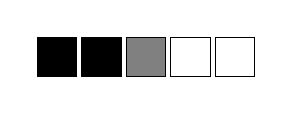
\begin{tikzpicture}
      \matrix (states) [strip, ampersand replacement=\&] {
        |[comp]| \& |[comp]| \& |[partial]| \& |[uncomp]| \& |[uncomp]| \\
      };
    \end{tikzpicture}

    but not

    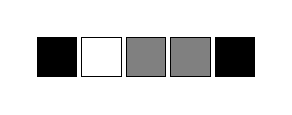
\begin{tikzpicture}
      \matrix (states) [strip, ampersand replacement=\&] {
        |[comp]| \& |[uncomp]| \& |[partial]| \& |[partial]| \& |[comp]| \\
      };
    \end{tikzpicture}
  \end{center}

  \begin{equation*}
    \FlaTwoByOne{\statepicflame{fusecond-1-t}{comp}}{\statepicflame{fusecond-1-b}{partial}}
    ;
    \FlaTwoByOne{\statepicflame{fusecond-2-t}{comp}}{\statepicflame{fusecond-2-b}{uncomp}}
  \end{equation*}
  \begin{tikzpicture}[remember picture, overlay]
    \path[->] (fusecond-1-b.east) edge [thick, bend left] (fusecond-2-t.west);
  \end{tikzpicture}
\end{frame}

\begin{frame}
  \frametitle{Cholesky + lower-triangular solve}
  \begin{columns}
    \begin{column}[t]{0.45\textwidth}
      Cholesky invariants.
      \begin{align*}
        &{\FlaTwoByTwo{L_{TL} = CHOL(\hat{L}_{TL})}{*}
          {L_{BL} = \hat{L}_{BL}}{L_{BR} = \hat{L}_{BR}}}\\
        &\FlaTwoByTwo{L_{TL} = CHOL(\hat{L}_{TL})}{*}
          {L_{BL} = \hat{L}_{BL}\widetilde{L}_{TL}^{-T}}{L_{BR} = \hat{L}_{BR}}\\
        &{\small \FlaTwoByTwo{L_{TL} = CHOL(\hat{L}_{TL})}{*}
          {L_{BL} = \hat{L}_{BL}\widetilde{L}_{TL}^{-T}}{L_{BR} = \hat{L}_{BR} - \widetilde{L}_{BL}\widetilde{L}_{BL}^T}}
      \end{align*}
    \end{column}
    \begin{column}[t]{0.55\textwidth}
      Lower triangular solve algorithms
      \begin{align*}
        &\FlaTwoByOne{B_T = L_{TL} \setminus \hat{B}_T}{B_B = \hat{B}_B}\\
        &{\FlaTwoByOne{B_T = L_{TL} \setminus \hat{B}_T}{B_B = \hat{B}_B - L_{BL}\widetilde{B}_T}}
      \end{align*}
    \end{column}
  \end{columns}

  Six cases to check ($3 \times 2$).
\end{frame}

\begin{frame}
  \frametitle{Cholesky + solve: easy cases}
  \textbf{TODO, should these be invariants or state pictures or both?}

  \begin{columns}
    \begin{column}[t]{0.45\textwidth}
      Cholesky invariants.
      \begin{align*}
        &\FlaTwoByTwo{L_{TL} = CHOL(\hat{L}_{TL})}{*}
          {L_{BL} = \hat{L}_{BL}\widetilde{L}_{TL}^{-T}}{L_{BR} = \hat{L}_{BR}}\\
        &\text{or}\\
        &{\small \FlaTwoByTwo{L_{TL} = CHOL(\hat{L}_{TL})}{*}
          {L_{BL} = \hat{L}_{BL}\widetilde{L}_{TL}^{-T}}{L_{BR} = \hat{L}_{BR} - \widetilde{L}_{BL}\widetilde{L}_{BL}^T}}
      \end{align*}
    \end{column}
    \begin{column}[t]{0.55\textwidth}
      Lower triangular solve algorithms
      \begin{align*}
        &\FlaTwoByOne{B_T = L_{TL} \setminus \hat{B}_T}{B_B = \hat{B}_B}\\
        &\text{and}\\
        &{\FlaTwoByOne{B_T = L_{TL} \setminus \hat{B}_T}{B_B = \hat{B}_B - L_{BL}\widetilde{B}_T}}
      \end{align*}
    \end{column}
  \end{columns}

  \begin{itemize}
  \item Greediest algorithm needs $L_{TL}$ and $L_{BL}$
  \item Both these Cholesky algorithms fully compute them
  \end{itemize}
\end{frame}

\begin{frame}
  \frametitle{Cholesky + solve, remaining cases}
    \begin{columns}
    \begin{column}[t]{0.45\textwidth}
      Cholesky invariants.
      \begin{align*}
        &{\FlaTwoByTwo{L_{TL} = CHOL(\hat{L}_{TL})}{*}
          {L_{BL} = \hat{L}_{BL}}{L_{BR} = \hat{L}_{BR}}}
      \end{align*}
    \end{column}
    \begin{column}[t]{0.55\textwidth}
      Lower triangular solve algorithms
      \begin{align*}
        &\FlaTwoByOne{B_T = L_{TL} \setminus \hat{B}_T}{B_B = \hat{B}_B}\\
        &\text{and}\\
        &\mathbf{\FlaTwoByOne{B_T = L_{TL} \setminus \hat{B}_T}{B_B = \hat{B}_B - L_{BL}\widetilde{B}_T}}
      \end{align*}
    \end{column}
  \end{columns}

  \begin{itemize}
  \item Can't fuse with second solve algorithm ($L_{BL}$ unavailable)
  \item So, five fusable algorithms
  \end{itemize}
\end{frame}

\begin{frame}
  \frametitle{Cholesky + lower solve + upper solve}
  \begin{itemize}
  \item Can't add $L^T \setminus B$
  \item We'd need $L^T_{BR}$, which is never fully computed
  \item Would also need to write on $B_B$
  \item Doesn't work even with temporary variables
  \end{itemize}

  \begin{equation*}
    \FlaTwoByTwo{\statepic{comp}}{*}{\statepic{comp}}{\statepic{partial}}
    ;
    \FlaTwoByOne{\statepic{comp}}{\statepic{partial}}
    ;
    \FlaTwoByOne{\statepic{uncomp}}{\statepic{comp}}
  \end{equation*}
\end{frame}

\section{Implementation}

\frame{\sectionpage}

\begin{frame}
  \frametitle{Tasks}
  \begin{itemize}
  \item Need to show software where partial computations can happen
  \item Pull suboperations that overwrite region into own names
  \item $\coloneqq_O$ is operation we want to do
  \end{itemize}
  \begin{equation*}
    \FlaTwoByTwo{\widetilde{A}_{TL} \coloneqq_O CHOL(\hat{A}_{TL})}{*}
    {\widetilde{A}_{BL} \coloneqq \hat{A}_{BL}\widetilde{A}_{TL}^{-T}}
    {\begin{array}{c}
       A_{BR, 0} \coloneqq \hat{A}_{BR} - \widetilde{A}_{BL}\widetilde{A}_{BL}^T;\\
       \widetilde{A}_{BR} \coloneqq_O CHOL(A_{BR, 0})
     \end{array}}
 \end{equation*}

 \begin{equation*}
   \FlaTwoByOne{\widetilde{B}_T \coloneqq_O L_{TL} \setminus \hat{B}_T}
   {\begin{array}{c}
      B_{B, 0} \coloneqq \hat{B}_B - L_{BL}\widetilde{B}_T;\\
      \widetilde{B}_B \coloneqq_O L_{BR} \setminus B_{B, 0}
    \end{array}}
 \end{equation*}
\end{frame}

\begin{frame}
  \frametitle{Working in either order}
  \begin{itemize}
  \item $\widetilde{A} = \hat{A} - B - C$ can be:
    \begin{itemize}
    \item $A_0 \coloneqq \hat{A} - B; \widetilde{A} \coloneqq A_0 - C$ or
    \item $A_0 \coloneqq \hat{A} - C; \widetilde{A} \coloneqq A_0 - B$
    \end{itemize}

  \item Sometimes we want to consider both cases (like in Sylvester equations)
  \item Add new temporary type, $A_{R, (n, x)}$
  \item Now we can write
    \begin{align*}
      A_{(0, a)} &\coloneqq (\hat{A} \vee A_{(0, b)}) - B;
      A_{(0, b)} &\coloneqq (\hat{A} \vee A_{(0, a)}) - B
    \end{align*}
  \item With this, computed is all tasks in remainder and so on
  \end{itemize}
\end{frame}

\begin{frame}
  \frametitle{Dependencies, v2}
  \begin{itemize}
  \item Name $\hat{A}_R$ as $\hat{A}_{R, \bot}$ and $\widetilde{A}$ as $A_{R, \top}$
  \item $A_{R, \sigma}$ is before (can compute) $A_{R', \sigma'}$ if:
    \begin{itemize}
    \item $R \neq R'$ (different regions) or
    \item $\sigma$ can reach $\sigma'$ on
      \begin{equation*}
        \begin{array}{c c c c c c c c c}
           & &(0, x)&\to&(1, x)&\to&\cdots& &\\
           & &\updownarrow     & &\updownarrow     &\to&\updownarrow& &\\
          \bot&\to&0     &\to&1     &\to&\cdots&\to&\top\\
           & &\updownarrow     & &\updownarrow     &\to&\updownarrow& &\\
           & &(0, y)&\to&(1, y)&\to&\cdots& &\\
        \end{array}
      \end{equation*}
    \end{itemize}
  \item If anything from an or is before, all of it is
  \end{itemize}
\end{frame}

\begin{frame}
  \frametitle{Finding all loop invariants}
  \begin{itemize}
  \item For each invariant/remainder split:
    \begin{itemize}
    \item Ensure operation task ($\coloneqq_O$) in invariant and remainder
    \item All inputs to invariant tasks must be before all remainder task outputs (no using data you don't have)
    \item All invariant task outputs must be before all remainder task inputs (no overwriting data you'll need)
    \end{itemize}
  \end{itemize}
\end{frame}

\begin{frame}
  \frametitle{Fusion works differently}
  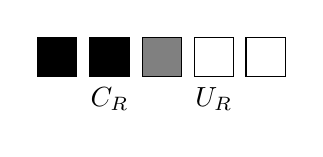
\begin{tikzpicture}
      \matrix (states) [strip, ampersand replacement=\&] {
        |[comp]| \& |[comp,label={below:$C_R$}]| \& |[partial]| \& |[uncomp,label={below:$U_R$}]| \& |[uncomp]| \\
      };
  \end{tikzpicture}

  \begin{itemize}
  \item While searching, add constraints to $C_R$s and $U_R$s
  \item $A_R$ read in invariant $i$ $\Rightarrow$ $C_R \geq i - 1$
  \item $A_R$ read in remainder $i$ $\Rightarrow$ $U_R \leq i + 1$
  \item Translates conditions from earlier
  \item If constraints fail, unwind search
  \end{itemize}
\end{frame}

\begin{frame}
  \frametitle{Multiple matrices}
  \begin{itemize}
  \item Need to add empty regions so all strips are same length
  \item Slight change to constraint system
  \end{itemize}

  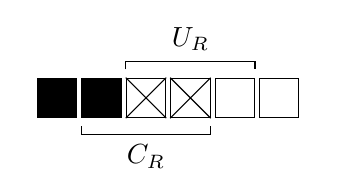
\begin{tikzpicture}
    \matrix (strip) [strip, ampersand replacement=\&] {
      |[comp]| \& |[comp]| \& |[uncomp]| \& |[uncomp]| \& |[uncomp]| \& |[uncomp]|\\
    };
    \emptyreg{strip-1-3};
    \emptyreg{strip-1-4};
    \bracelabel{strip-1-2.south west}{strip-1-4.south east}{below}{$C_R$};
    \bracelabel{strip-1-3.north west}{strip-1-5.north east}{above}{$U_R$};
  \end{tikzpicture}
\end{frame}

\begin{frame}
  \frametitle{Comes from task}
  \begin{itemize}
  \item For things like $LU = A$, tasks write multiple regions
  \item To prevent duplicates, use $U_R \leftarrow L_R$ (comes from)
  \item If $L_R$ computed, $U_R$ is computed, otherwise not
  \end{itemize}
\end{frame}

\section{Demo}

\frame{\sectionpage}

\begin{frame}
  \frametitle{Another important example}
  \begin{itemize}
  \item Graph problem $C = (AM + (AM)^T) - MM$, where $A$ and $M$ are symmetric
  \item $C \coloneqq (AM + (AM)^T); C \coloneqq C - MM$ has $56$ fused algorithms
  \item However, $A \coloneqq (AM + (AM)^T); A \coloneqq A - MM$ has no algorithms
  \end{itemize}
\end{frame}

\begin{frame}
  \frametitle{Demo time}
\end{frame}

\section{Experiments}

\begin{frame}
  \frametitle{TODO do an experiment?}
\end{frame}

\section{Conclusions}

\begin{frame}
  \frametitle{Conclusions}
  \begin{itemize}
  \item We can automatically find fusable loop invariants
  \item This is often helpful
  \item This analysis needs to be at this level
  \end{itemize}
\end{frame}

\begin{frame}
  \frametitle{Acknowledgments}
  \begin{itemize}
  \item Tze Meng for doing all the theory
  \end{itemize}
\end{frame}

\begin{frame}
  \frametitle{Future work}
  \begin{itemize}
  \item Probably not --- maybe codegen
  \end{itemize}
\end{frame}

\section*{The old slides}

\begin{frame}
  \frametitle{High-level loop fusion}
  \begin{itemize}
  \item Problems often are a series of subproblems
  \item Combining subalgorithms often helps performance
  \item Goal: find all the fused algorithms for a problem
  \item Compilers know too many details - need a high level approach
  \end{itemize}
\end{frame}

\begin{frame}
  \frametitle{FLAME algorithms, loop invariants}
  \begin{itemize}
  \item FLAME = Formal Linear Algebra Methods Eenvironments
  \item Provably correct algorithms from spec
  \item Algorithms $\Leftrightarrow$ loop invariants
  \item We know how to:
    \begin{itemize}
    \item Autogenerate algorithm/code from loop invariant
    \item Autogenerate all possible loop invariants
    \item Identify when fusion is possible (in theory)
    \end{itemize}
  \end{itemize}
\end{frame}

\begin{frame}
  \frametitle{What we add}
  \begin{itemize}
  \item Autogenerate all sets of fusable loop invariants
  \item Input is \emph{partitioned matrix expression} --- indicates needed computations
  \item Can be used to generate code
  \end{itemize}
\end{frame}

\section{FLAME}

\frame{\sectionpage}

\begin{frame}
  \frametitle{Goal}
  Want to compute
  \begin{columns}
    \begin{column}{0.5\textwidth}
      \begin{equation*}
        \widetilde{A} = \opF(\hat(A), \underbrace{\ldots}_{O})
      \end{equation*}
    \end{column}
    \begin{column}{0.5\textwidth}
      \begin{equation*}
        \widetilde{A} = CHOL(\hat{A})
      \end{equation*}
    \end{column}
  \end{columns}

  $\hat{A}$ and $\widetilde{A}$ share memory ($A$).

  Initially, $A = \hat{A}$.

  At termination, $A = \widetilde{A}$.
\end{frame}

\begin{frame}
  \frametitle{Algorithm structure}
  \begin{FlameAlg}
    \FlaPartition{ $A \rightarrow \FlaTwoByTwo{A_{TL}}{A_{TR}}{A_{BL}}{A_{BR}}$}{\\
      $\quad$ where $\operatorname{dim}(A_{TL}) = 0 \times 0$}\\
    \FlaDoUntil{ $\operatorname{dim}(A_{TL}) = n \times n$}\\
    \FlaRepartition{$\FlaTwoByTwo{A_{TL}}{A_{TR}}{A_{BL}}{A_{BR}}%
      \rightarrow \FlaThreeByThreeBR{A_{00}}{a_{01}}{A_{02}}%
      {a_{10}^T}{\alpha_{11}}{a_{12}^T}%
      {A_{02}}{a_{21}}{A_{22}}$}\\
    $\?[\vdots]\text{ loop body}$\\ % Make the balanced braces check shut up
    \FlaContinue{$\FlaTwoByTwo{A_{TL}}{A_{TR}}{A_{BL}}{A_{BR}} \leftarrow{}%
      \FlaThreeByThreeTL{A_{00}}{a_{01}}{A_{02}}%
      {a_{10}^T}{\alpha_{11}}{a_{12}^T}%
      {A_{20}}{a_{21}}{A_{22}}$}\\
    \FlaEndDo{}
  \end{FlameAlg}
\end{frame}

\begin{frame}
  \frametitle{Algoriithm example}
  \begin{FlameAlg}
    \FlaPartition{ $A \rightarrow \FlaTwoByTwo{A_{TL}}{*}{A_{BL}}{A_{BR}}$}{\\
      $\quad$ where $\operatorname{dim}(A_{TL}) = 0 \times 0$}\\
    \FlaDoUntil{ $\operatorname{dim}(A_{TL}) = n \times n$}\\
    \FlaRepartition{$\FlaTwoByTwo{A_{TL}}{*}{A_{BL}}{A_{BR}}%
      \rightarrow \FlaThreeByThreeBR{A_{00}}{*}{*}%
      {a_{10}^T}{\alpha_{11}}{*}%
      {A_{02}}{a_{21}}{A_{22}}$}\\
    $\alpha_{11} \coloneqq \sqrt{\alpha_{11}}$\\
    $a_{21} \coloneqq a_{21} / \alpha_{11}$\\
    $A_{22} \coloneqq A_{22} - a_{21}a_{21}^T$\\
    \FlaContinue{$\FlaTwoByTwo{A_{TL}}{*}{A_{BL}}{A_{BR}} \leftarrow{}%
      \FlaThreeByThreeTL{A_{00}}{*}{*}%
      {a_{10}^T}{\alpha_{11}}{*}%
      {A_{20}}{a_{21}}{A_{22}}$}\\
    \FlaEndDo{}
  \end{FlameAlg}
\end{frame}

\begin{frame}
  \frametitle{Partitioned Matrix Expressions}
  \begin{itemize}
  \item Take $A$ (and maybe other stuff), split it into regions.
  \item Lines between regions move during algorithm
  \end{itemize}
  \begin{equation*}
    \FlaTwoByTwo{\widetilde{A}_{TL} = \opF_{TL}(\hat{A}, \ldots)}{\widetilde{A}_{TR} = \opF_{TR}(\hat{A}, \ldots)}
    {\widetilde{A}_{BL} = \opF_{BL}(\hat{A}, \ldots)}{\widetilde{A}_{BR} = \opF_{BR}(\hat{A}, \ldots)}
  \end{equation*}

  \begin{equation*}
    \FlaTwoByTwo{\widetilde{A}_{TL} = CHOL(\hat{A}_{TL})}{*}
    {\widetilde{A}_{BL} = \hat{A}_{BL}\widetilde{A}_{TL}^{-T}}
    {\widetilde{A}_{BR} = CHOL(\hat{A}_{BR} - \widetilde{A}_{BL}\widetilde{A}_{BL}^T)}
  \end{equation*}
\end{frame}

\begin{frame}
  \frametitle{Loop invariants}
  \begin{itemize}
  \item Find $\opf_R$ and $\opf'_R$ so $\opF_R(\hat{A}) = \opf'(\opf(\hat{A}))$.
  \item $\opf_R$ is loop invariant for $R$, $\opf'_R$ is remainder
  \item Invariant for algorithm is an invariant per region
  \item Completely determine algorithm
  \end{itemize}
\end{frame}

\begin{frame}
  \frametitle{This is a loop invariant}
  Starting from Cholesky's PME:
  \begin{equation*}
    \FlaTwoByTwo{\widetilde{A}_{TL} = CHOL(\hat{A}_{TL})}{*}
    {\widetilde{A}_{BL} = \hat{A}_{BL}\widetilde{A}_{TL}^{-T}}
    {\widetilde{A}_{BR} = CHOL(\hat{A}_{BR} - \widetilde{A}_{BL}\widetilde{A}_{BL}^T)}
  \end{equation*}

  We obtain
  \begin{equation*}
    \FlaTwoByTwo{A_{TL} = CHOL(\hat{A}_{TL})}{*}
    {A_{BL} = \hat{A}_{BL}\widetilde{A}_{TL}^{-T}}
    {A_{BR} = \hat{A}_{BR} - \widetilde{A}_{BL}\widetilde{A}_{BL}^T}
  \end{equation*}
\end{frame}

\begin{frame}
  \frametitle{As are these}
  \begin{equation*}
    \FlaTwoByTwo{A_{TL} = CHOL(\hat{A}_{TL})}{*}
    {A_{BL} = \hat{A}_{BL}\widetilde{A}_{TL}^{-T}}
    {A_{BR} = \hat{A}_{BR}}
  \end{equation*}

  \begin{equation*}
    \FlaTwoByTwo{A_{TL} = CHOL(\hat{A}_{TL})}{*}
    {A_{BL} = \hat{A}_{BL}}
    {A_{BR} = \hat{A}_{BR}}
  \end{equation*}
\end{frame}

\begin{frame}
  \frametitle{But not these}
  \begin{equation*}
    \FlaTwoByTwo{A_{TL} = CHOL(\hat{A}_{TL})}{*}
    {A_{BL} = \hat{A}_{BL}\widetilde{A}_{TL}^{-T}}
    {A_{BR} = CHOL(\hat{A}_{BR} - \widetilde{A}_{BL}\widetilde{A}_{BL}^T)}
  \end{equation*}

  \begin{equation*}
    \FlaTwoByTwo{A_{TL} = \hat{A}_{TL}}{*}
    {A_{BL} = \hat{A}_{BL}}
    {A_{BR} = \hat{A}_{BR}}
  \end{equation*}
\end{frame}

\begin{frame}
  \frametitle{Or this}
  \begin{equation*}
    \FlaTwoByTwo{A_{TL} = \hat{A}_{TL}}{*}
    {A_{BL} = \hat{A}_{BL}\widetilde{A}_{TL}^{-T}}
    {A_{BR} = \hat{A}_{BR}}
  \end{equation*}
\end{frame}

\begin{frame}
  \frametitle{Tasks}
  \begin{itemize}
  \item We need to specify split points
  \end{itemize}

  \begin{equation*}
    \FlaTwoByTwo{\widetilde{A}_{TL} \coloneqq_O CHOL(\hat{A}_{TL})}{*}
    {\widetilde{A}_{BL} \coloneqq \hat{A}_{BL}\widetilde{A}_{TL}^{-T}}
    {\begin{array}{c}
       A_{BR, 0} \coloneqq \hat{A}_{BR} - \widetilde{A}_{BL}\widetilde{A}_{BL}^T;\\
       \widetilde{A}_{BR} \coloneqq_O CHOL(A_{BR, 0})
     \end{array}}
  \end{equation*}

  \begin{equation*}
    \FlaTwoByTwo{\widetilde{A}_{TL} \coloneqq_O \hat{A}_{TL}^{-1}}{*}
    {\begin{array}{c}
       A_{BL, (0, a)} \coloneqq (\hat{A}_{BL} \vee A_{BL, (0, b)}) \cdot \widetilde{A}_{TL};\\
       A_{BL, (0, b)} \coloneqq -\hat{A}_{BR}^{-1} \cdot (\hat{A}_{BL} \vee A_{BL, (0, a)})
     \end{array}}
    {\widetilde{A}_{BR} \coloneqq_O \hat{A}_{BR}^{-1}}
  \end{equation*}
\end{frame}

\begin{frame}
  \frametitle{More abstractly}
  The code translates tasks to

    \begin{equation*}
    \FlaTwoByTwo{A_{TL, \top} \coloneqq_O \{A_{TL, \bot}\}}{*}
    {A_{BL, \top} \coloneqq \{A_{BL, \bot}, A_{TL, \top}\}}
    {\begin{array}{c}
       A_{BR, 0} \coloneqq \{A_{BR, \bot}\, A_{BL, \top};\\
       A_{BR, \top} \coloneqq_O \{A_{BR, 0}\}
     \end{array}}
  \end{equation*}

  \begin{equation*}
    \FlaTwoByTwo{A_{TL, \top} \coloneqq_O \{A_{TL, \bot}}{*}
    {\begin{array}{c}
       A_{BL, (0, a)} \coloneqq \{A_{BL, \bot} \vee A_{BL, (0, b)}, A_{TL, \top}\};\\
       A_{BL, (0, b)} \coloneqq \{A_{BR, \bot}, A_{BL, \bot} \vee A_{BL, (0, a)}\}
     \end{array}}
    {A_{BR, \top} \coloneqq_O \{A_{BR, \bot}\}}
  \end{equation*}
\end{frame}

\begin{frame}
  \frametitle{Dependencies, v2}
  \begin{itemize}
  \item $A_{R, \sigma}$ is before (can compute) $A_{R', \sigma'}$ if:
    \begin{itemize}
    \item $R \neq R'$ (different regions) or
    \item
      \begin{equation*}
        \begin{array}{c c c c c c c c c}
           & &(0, x)&\to&(1, x)&\to&\cdots& &\\
           & &\updownarrow     & &\updownarrow     &\to&\updownarrow& &\\
          \bot&\to&0     &\to&1     &\to&\cdots&\to&\top\\
           & &\updownarrow     & &\updownarrow     &\to&\updownarrow& &\\
           & &(0, y)&\to&(1, y)&\to&\cdots& &\\
        \end{array}
      \end{equation*}
    \end{itemize}
  \item If anything from an or is before, all of it is
  \end{itemize}
\end{frame}

\begin{frame}
  \frametitle{Dependency validity}
  \begin{itemize}
  \item Invariant/remainder split has valid dependencies if:
    \begin{itemize}
    \item All past task inputs before all future task outputs
    \item All past task outputs not after all future task inputs
    \end{itemize}
  \end{itemize}
\end{frame}

\begin{frame}
  \frametitle{Finding all invariants}
  \begin{enumerate}
  \item Pick a past/future split for each region
  \item Check if the loop can make progress
  \item Check for dependency validity
  \end{enumerate}
\end{frame}

\section{Loop fusion}

\frame{\sectionpage}

\begin{frame}
  \frametitle{States of a region}
  \begin{description}
  \item[Fully computed] All tasks in the invarient
  \item[Uncomputed] All tasks in the remainder
  \item[Partially computed] Everything else
  \end{description}
\end{frame}

\begin{frame}
  \frametitle{The fusion problem}
  \begin{equation*}
    \begin{rcases}
      \widetilde{A}^0 &= \opF^0(\hat{A}^0)\\
      \widetilde{A}^1 &= \opF^1(\hat{A}^1)\\
      &\vdots\\
      \widetilde{A}^{n - 1} &= \opF^{n - 1}(\hat{A}^{n - 1})
    \end{rcases} \widetilde{A}^{n - 1} = \opF(\hat{A}^0)
  \end{equation*}
  where $\hat{A}^{i + 1} = \widetilde{A}^i$
\end{frame}

\begin{frame}
  \frametitle{Fusion conditions}
  \begin{equation*}
    \hat{A}^{i + 1}_{\mathbf{R}} = \widetilde{A}_{\mathbf{R}}^i \text{ \textbf{if needed}}
  \end{equation*}

  \begin{itemize}
  \item $\opF^i$'s invariant needs $R$ $\Rightarrow$ $\opF^{j < i}_R$ fully computed
  \item $\opF^i$'s remainder needs $R$ $\Rightarrow$ $\opF^{j > i}_R$ uncomputed
  \end{itemize}
\end{frame}

\begin{frame}
  \frametitle{An example: Cholesky + lower-triangular solve}
  \begin{columns}
    \begin{column}{0.5\textwidth}
      Cholesky algorithms.
      \begin{align*}
        &\alt<2->{\cancel{\FlaTwoByTwo{L_{TL} = CHOL(\hat{L}_{TL})}{*}
          {L_{BL} = \hat{L}_{BL}}{L_{BR} = \hat{L}_{BR}}}}
          {\FlaTwoByTwo{L_{TL} = CHOL(\hat{L}_{TL})}{*}
          {L_{BL} = \hat{L}_{BL}}{L_{BR} = \hat{L}_{BR}}}\\
        &\FlaTwoByTwo{L_{TL} = CHOL(\hat{L}_{TL})}{*}
          {L_{BL} = \hat{L}_{BL}\widetilde{L}_{TL}^{-T}}{L_{BR} = \hat{L}_{BR}}\\
        &\FlaTwoByTwo{L_{TL} = CHOL(\hat{L}_{TL})}{*}
          {L_{BL} = \hat{L}_{BL}\widetilde{L}_{TL}^{-T}}{L_{BR} = \hat{L}_{BR} - \widetilde{L}_{BL}\widetilde{L}_{BL}^T}\\
      \end{align*}
    \end{column}
    \begin{column}{0.5\textwidth}
      Lower triangular solve algorithms
      \begin{align*}
        &\FlaTwoByOne{B_T = L_{TL} \setminus \hat{B}_T}{B_B = \hat{B}_B}\\
        &\alt<2->{\cancel{\FlaTwoByOne{B_T = L_{TL} \setminus \hat{B}_T}{B_B = \hat{B}_B - L_{BL}\widetilde{B}_T}}}
        {\FlaTwoByOne{B_T = L_{TL} \setminus \hat{B}_T}{B_B = \hat{B}_B - L_{BL}\widetilde{B}_T}}\\
      \end{align*}
    \end{column}
  \end{columns}

  5 fused algorithms. (All combinations fuse except one.)
\end{frame}

\begin{frame}
  \frametitle{We can't go further}
  Consider:
  \begin{align*}
    L &\coloneqq CHOL(L) & \FlaTwoByTwo{\widetilde{A}_{TL} \coloneqq_O CHOL(\hat{A}_{TL})}{*}
                           {\widetilde{A}_{BL} \coloneqq \hat{A}_{BL}\widetilde{A}_{TL}^{-T}}
                           {\begin{array}{c}
                              A_{BR, 0} \coloneqq \hat{A}_{BR} - \widetilde{A}_{BL}\widetilde{A}_{BL}^T;\\
                              \widetilde{A}_{BR} \coloneqq_O CHOL(A_{BR, 0})
                            \end{array}}\\
    T &\coloneqq L^{-1}B & \FlaTwoByOne{\widetilde{T}_T \coloneqq_O TRSV(\hat{L}_{TL}, B_T)}
                             {\begin{array}{c}
                                T_{B, 0} \coloneqq \hat{T}_B - \hat{L}_{BL}\widetilde{T}_T\\
                                \widetilde{T}_B \coloneqq_O TRSV(\hat{L}_{BR}, T_{B, 0})
                              \end{array}}\\
    X &\coloneqq L^{-T}B & \FlaTwoByOne{
                           \begin{array}{c}
                             X_{T, 0} \coloneqq \hat{X}_T - \hat{L}^T_{BL}\widetilde{X}_B\\
                             \widetilde{X}_T \coloneqq_O TRSV(\hat{L}_{BR}, X_{T, 0})
                           \end{array}}
    {X_B \coloneqq TRSV(\hat{L}_{BR}, \hat{T}_B)}\\
  \end{align*}

  \begin{itemize}
  \item No fused algorithm (we checked)
  \item Top to bottom vs. bottom to top
  \end{itemize}
\end{frame}

\begin{frame}
  \frametitle{Strips}
  \begin{itemize}
  \item Strip: sequence of region $R$ from each loop
  \item Potentially fusable strip has:
    \begin{itemize}
    \item Some number of fully computed regions, then
    \item Optionally, one partially computed region, then
    \item Uncomputed regions
    \end{itemize}
  \end{itemize}

  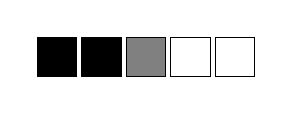
\begin{tikzpicture}
    \matrix (states) [strip, ampersand replacement=\&] {
      |[comp]| \& |[comp]| \& |[partial]| \& |[uncomp]| \& |[uncomp]| \\
    };
  \end{tikzpicture}

  but not

  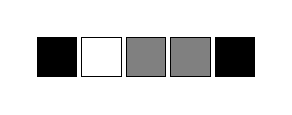
\begin{tikzpicture}
    \matrix (states) [strip, ampersand replacement=\&] {
      |[comp]| \& |[uncomp]| \& |[partial]| \& |[partial]| \& |[comp]| \\
    };
  \end{tikzpicture}
\end{frame}

\begin{frame}
  \frametitle{Finding fusable loops}
  \begin{itemize}
  \item Search through potentially fusable strips
    \begin{itemize}
    \item
      
\begin{tikzpicture}
        \matrix (states) [strip, row sep=0.1cm, ampersand replacement=\&] {
          |[comp, label={below:Any}]| \& |[uncomp]| \& |[rectangle=no,draw=white]| $=$ \& |[comp]| \& |[uncomp,label={below:Any}]|\\
        };
      \end{tikzpicture}
    \end{itemize}
  \item Enforce fusion constraints throughout
  \item Check all fusable strip-sets to see if each loop has an invariant
  \end{itemize}
\end{frame}

\begin{frame}
  \frametitle{Last computed, first uncomputed}
  \begin{itemize}
  \item Track constraints on last computed region $C_R$ (and first uncomptued $U_R$)
  \item Initially, $-1 \leq C_R, U_R \leq n$ (maybe nothing/everything is computed/uncomputed)
  \item Past read in loop $i$: $C_R \geq i - 1$
  \item Future read in loop $i$: $U_R \leq i + 1$
  \item When strip is made, set $C_R$ and $U_R$, add more constraints
  \item On failure, backtrack
  \end{itemize}
\end{frame}

\begin{frame}
  \frametitle{Multiple matrices}
  \begin{itemize}
  \item Some operations have multiple outputs
  \item (Ex. $y = Lx; L = L^{-1}$)
  \item All strips must be same length --- add empty regions
  \item De-dup check from before works
  \end{itemize}
\end{frame}

\begin{frame}
  \frametitle{Multiple matrices}
  \begin{itemize}
  \item Last computed or first uncomputed can be followed by empty
  \item If so, bound $\{C, U\}_R$ to include the empty regions
  \item Needed to make constraints work
  \end{itemize}
  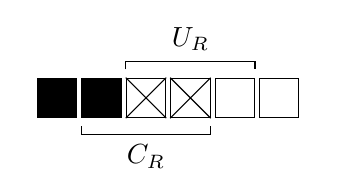
\begin{tikzpicture}
    \matrix (strip) [strip, ampersand replacement=\&] {
      |[comp]| \& |[comp]| \& |[uncomp]| \& |[uncomp]| \& |[uncomp]| \& |[uncomp]|\\
    };
    \emptyreg{strip-1-3};
    \emptyreg{strip-1-4};
    \bracelabel{strip-1-2.south west}{strip-1-4.south east}{below}{$C_R$};
    \bracelabel{strip-1-3.north west}{strip-1-5.north east}{above}{$U_R$};
  \end{tikzpicture}
\end{frame}

\begin{frame}
  \frametitle{Comes from task}
  \begin{itemize}
  \item For things like $LU = A$, tasks write multiple regions
  \item To prevent duplicates, use $U_R \leftarrow L_R$ (comes from)
  \item If $L_R$ computed, $U_R$ is computed, otherwise not
  \end{itemize}
\end{frame}

\begin{frame}
  \frametitle{Another important example}
  \begin{itemize}
  \item Graph problem $C = (AM + (AM)^T) - MM$, where $A$ and $M$ are symmetric
  \item $C \coloneqq (AM + (AM)^T); C \coloneqq C - MM$ has $56$ fused algorithms
  \item However, $C = A$ or $C = M$ gives $0$ algorithms
    \begin{itemize}
    \item Dependencies: $TL \leftrightarrow TR$ and $TR \leftrightarrow BR$
    \item Overwriting one quadrant requires computing everything
    \item \textbf{TODO figure}
    \end{itemize}
  \end{itemize}
\end{frame}

\end{document}
